%\documentclass[11pt]{article}
%\usepackage{graphicx}

%\begin{document}

\chapter{Bose-Einstein Condensation}
This chapter explores both a theoretical framework for forming Bose-Einstein Condensation as well as the experimental process on the atom chip based machine. 
\newline

\section{Theoretical Basis for Bose-Einstein Condensation}
This section will discuss the basics of Bose-Einstein statistics, introducing the quantum statistics that describe systems of bosons. Assuming a basis in Boltzmann statistics, the Bose-Einstein distribution is built. From there, the theoretical framework for the realization of Bose-Einstein Condensation will be examined. In this analysis, core concepts for Bose-Einstein Condensate formation will be reviewed including: de Broglie wavelength, critical temperature, and phase space density. 

\subsection{Maxwell-Boltzmann Statistics}
Recalling from Thermal Physics, Boltzmann statistics describe the probability that a particle occupies a state $s$ as
\beq
P_s = \frac{1}{\Zeta_1}e^{-E_s/kT}
\eeq
where $k$ is the Boltzmann constant, $E_s$ is the energy of the particle in state $s$, $\mathrm{Z}$ is the partition function, and $T$ is the temperature of the system. 
\newline
This leads to a partition function of the form 
\beq
\Zeta_1 = \sum_s{e^{-E_s/kT}}
\eeq 
in order to satisfy that the probability of finding the particle in any state is certain.
\beq
\sum_s{P_s}=\sum_s{\frac{1}{\Zeta_1}e^{-E_s/kT}} =\frac{\sum_s{e^{-E_s/kT}}}{\sum_s{e^{-E_s/kT}}}=1
\eeq


Likewise, Boltzmann statistics describe the probability that a system of $n$ particles will be found in state $s$ as 
\beq
P_s(n) = \frac{1}{\mathrm{Z}} e^{-n(\epsilon_s-\mu) /kT}
\eeq
where $k$ is the Boltzmann constant, $\epsilon_s$ is the energy of one particle in state $s$, $\Zeta$ is the partition function, $\mu$ is the chemical potential, and $T$ is the temperature of the system. This derivation comes from considering the entropy of different states of the system with its surroundings.

\subsection{Bose-Einstein Statistics}

Recall that bosons do not obey the Pauli-Exclusion principle. So, unlike fermions, $n$ can be any integer from $0$ to $\infty$. Considering this, we can find the partition function for these indistinguishable particles by making sure the probability of that state being occupied by any possible number of bosons is certain.
$$\mathrm{Z} = \sum_n{e^{-n(\epsilon_s-\mu) /kT}}= 1 + e^{-(\epsilon_s-\mu) /kT} + \left( e^{-(\epsilon_s-\mu) /kT} \right)^2 + ... $$
\beq
\mathrm{Z}= \frac{1}{1- e^{-(\epsilon_s-\mu) /kT}}
\eeq
\newline
The following calculates the average number of bosons in a particular energy state, $\bar{n}_s$,
$$\bar{n}_s = \sum_n{nP_s(n)} $$
\beq
\bar{n}_s = \frac{1}{e^{(\epsilon_s-\mu) /kT}-1}
\eeq
The derivation for this can be found in \textbf{Appendix A.1}. This equation is known as the Bose-Einstein distribution. This equation describes the average number of bosons occupying a given state. In the classical limit, with many particles and lots of energy, where quantization becomes obsolete, a Bose-Einstein distribution is equivalent to a Maxwell-Boltzmann distribution, as expected. However, as Einstein discovered, the two distributions vary drastically for low temperatures where quantum mechanics begins to take effect. 
\newline

\subsection{Bose-Einstein Condensates}

Bose-Einstein Condensation formation occurs when the bosons all cluster towards the ground state. Using the equation for a Bose-Einstein distribution, the average number of atoms in the ground state is 
\beq
\bar{N}_0 = \frac{1}{e^{(\epsilon_0-\mu) /kT}-1}
\eeq
where $\epsilon_0$ is the energy of a boson in the ground state. Evidently, the average number of bosons increases as the temperature decreases. This function is of interest when $N_0$ becomes large. 
An expression for the total number of bosons, is therefore
\beq
N = \sum_s{\frac{1}{e^{(\epsilon_s-\mu) /kT}-1}}
\eeq
Evaluating this sum as a continuous integral and solving it yields a solution only valid for low temperatures below what will be defined as the critical temperature, $T_C$. This evaluation uses $g(\epsilon)$, the density of the states, or the number of particle states per unit of energy, calculated by summing the total energy from each electron. This continuous integration is not valid for the ground state and therefore gives a result for the number of atoms in the excited states\cite{foot}.
%MAYBE PUT THIS DERIVATION IN THE APPENDIX
\beq
N_{excited} = 2.612\left( \frac{2\pi mkT}{h^2} \right)^{\frac{3}{2}}V
\eeq
\beq
T_C = 0.527 \frac{h^2}{2\pi mk}\left( \frac{N}{V} \right)^\frac{2}{3}
\eeq
\textbf{Equation 1.9} describes, for temperatures below the critical temperature, the most amount of bosons that can be in excited states. After which, added bosons, under a constant temperature and volume, will go to the ground state. Therefore, this critical temperature describes when bosons start to cascade towards the ground state. The expression for the number of bosons in the excited states can be rewritten as 
\beq
N_{excited} = \left( \frac{T}{T_C} \right)^\frac{3}{2}N
\eeq
Using this, the number of photons in the ground state can be calculated.
$$N = N_{excited} + N_0$$
\beq 
N_0 = \left( 1 - \left( \frac{T}{T_C} \right)^\frac{3}{2} \right) N
\eeq 
These equations are plotted in \textbf{Figure 1.1}.
\begin{figure}[h]
\begin{center}
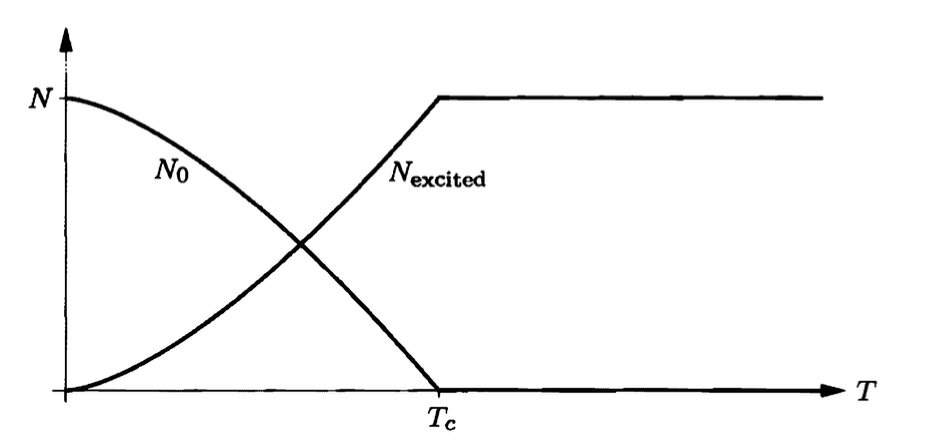
\epsfig{file=fig1_1.png}
\end{center}
\caption{The number of bosons in the excited and ground states.\cite{thermal} }
\end{figure}

Below the critical temperature, the bosons cascade down into the ground state. The number of bosons in the ground state, once below the critical temperature, grows by a factor of $T^{3/2}$ when the temperature decreases. At this point, most bosons share the same quantum state, $\psi$.
%%put figure of first bec from chu and cite?


Another way to think about Bose-Einstein condensation is through the de Broglie wavelength, which describes the wave-like nature of large particles. The thermal de Broglie wavelength, the de Broglie wavelength as a function of temperature, is
\beq 
\lambda_{T} = \frac{h}{\sqrt{2\pi Mk_B T}}
\eeq
At the point of Bose-Einsteins condensation, for Rubidium-87 atoms, like the ones we use in the Ultra-Cold Atom Lab at Bates, the wavelength of the atoms is significantly larger than their spacing or density. This means the wave-functions of the atoms overlap, creating a quantum effect that can be viewed on the scale of the atom cloud, which is about a few millimeters in the Ultra-Cold Lab. Therefore, another way to view the formation of Bose-Einstein condensation is through the phase space density of the bosons, $\rho$. The phase space density can be expressed as
\beq
\rho = n\lambda_T^3
\eeq
where $n$ is the number density of the bosons, or the average distance of a boson to one of its neighbors, and $\lambda_T$ describes the spread of the particles in terms of their wave-like properties. As before, the temperature must be lowered to increase the phase space density. As the thermal de Broglie wavelength grows by a factor of $T^{1/2}$ when the temperature is decreased, the phase space density grows by a factor of $T^{3/2}$. At low enough temperatures, the bosons become indistinguishable, this occurs when they are saturated in the ground state. At this point, the bosons form one 'super particle'. This 'super particle' is the Bose-Einstein Condensate. Its properties are intriguing due to their display of quantum mechanics on a macroscopic scale. Bose-Einstein Condensates can display interesting quantum phenomena such as the uncertainty principles, interference, and quantum tunneling.
\newline



\section{Experimental Process of Forming Bose-Einstein Condensation}

This section will focus on the basic instructions and concepts for forming a Bose-Einstein Condensate on the atom chip based Bose-Einstein Condensation machine in the Bates Ultra-Cold Atom Lab. This machine is referred to as the NASABEC machine due to its eventual goal to simulate experiments similar to the one on the International Space Station. This section will also serve as a basis for understanding the process and the future steps the Ultra-Cold Atom Lab must take. Other labs, including the Ultra-Cold Atom Lab at Bates, use different methods to form Bose-Einstein Condensates and study them. The general steps remain exceedingly similar and this section describes them in order. These general steps include laser cooling, optical pumping and magnetic trapping, and evaporative cooling. This section refrains from an exhaustive mathematical derivation for each step, though the following sources were used to create this section and can be further studied\cite{foot}\cite{metcalf_article}\cite{LCandT}.
\newline

\subsection{Why Rubidium-87?} 

The Ultra-Cold Atom lab uses Rubidium-87 to form Bose-Einstein Condensation. This is due to its unique properties of, of course, being a boson, its stability under low temperatures, and its simple atomic structure. Rubidium-87 has a positive scattering length meaning it is repulsive at low temperatures. Therefore, Rubidium-87 can be confined at low temperatures. Atoms with a negative scattering length, like the more abundant Rubidium-85 would be attracted to each other at these temperatures, violently colliding, and being sent out of the trap. 


In addition to a negative scattering length, Rubidium-87, and many other alkali metals, remain a vapour at these extremely low temperatures required to form a Bose-Einstein Condensate, which was long doubted by scientists. The process of Rubidium-87 forming a metal occurs on a time scale much longer than that necessary to form a Bose-Einstein Condensate. 


The final reason for using Rubidium-87 in Bose-Einstein Condensation formation is due to its simple atomic level structure. Rubidium-87 only has one valence electron. This makes its energy level structure quite simple for the purpose of exciting the valence electron. In addition, the transition of interest, $| F=2\rangle \rightarrow | F=3\rangle$, is a transition with an energy level difference that is quite easy to get relatively cheap lasers for. 


\subsection{Laser Cooling}

Laser cooling is the process of using a laser to drive transitions in atoms and using the recoil energy to slow the atom. Laser cooling uses concepts such as the Doppler effect, the Zeeman effect, and the energy structure of the Rubidium-87 atoms. Laser cooling is the first step in the process of cooling the atoms. To get Rubidium vapor, a piece of Rubidium metal is heated so that atoms sublimate off to be laser cooled. 

The basics behind laser cooling is to use the momentum of many photons to slow down an atom to a limit on the order of the momentum of the photons. On average, the force of one scatter on an atom is equal to the momentum of the absorbed photon. This is because the atom can release the absorbed photon in any direction which, on average, results in a net zero change in momentum for the atom.
\beq
F_{rad} = \frac{IA}{c}
\eeq
The scattering rate for a single atom is given by 
\beq
R_{scatt} = \frac{\Gamma}{2} \frac{\frac{I}{I_{sat}}}{1 + \frac{I}{I_{sat}} + 4 \left( \frac{\delta}{\Gamma}\right)^2 } 
\eeq
\beq 
F_{scatt} = \hbar k  \frac{\Gamma}{2} \frac{\frac{I}{I_{sat}}}{1 + \frac{I}{I_{sat}} + 4 \left( \frac{\delta}{\Gamma}\right)^2 } 
\eeq

where $\Gamma$ is the natural linewidth associated with the excited state, $I$ is the intensity of the laser, $I_{sat}$ is the saturation intensity defined by the transition the atom is being driven between, $k$ is the wave number of the light, and $\delta$ is the frequency detuning of the laser light from the resonant frequency, or the frequency that define the energy level difference in the transition the atom is being driven between. From \textbf{Equation 1.16} it is clear that increasing the intensity of the laser increases the scattering rate, though there is a maximum scattering rate of $\frac{\Gamma}{2}$ as the intensity approaches infinity. For this reason, lasers with output intensities much larger than the saturation intensity are not significantly more beneficial, making them undesired due to their steep costs. 


The frequency detuning can be expressed as
\beq
\delta = \omega - \omega_0 + k \nu
\eeq
where $\omega$ is the frequency of the light coming from the laser, $\omega_0$ is the resonant frequency for the transition, and $k\nu$ is the frequency shift of the light due to the Doppler effect. $k$ is the wave-number of the radiation, and $\nu$ is the velocity of the atom. The Doppler shift must be taken into account, because as atom are slowed, the original frequency they saw becomes off resonance; therefore, absorptions and further cooling becomes infeasible. This is discussed further in the context of the NASABEC machine later.  


To slow atoms, one might consider a pairs of orthogonal, counter-propagating beams as shown in \textbf{Figure 1.2}. One might red-detune the laser frequencies ($\omega < \omega_0$) so that atoms moving toward a laser, due to the Doppler shift, will be more likely to scatter light. This set up provides what is known as optical molasses. A set up of optical molasses is shown in \textbf{Figure 1.2}


\begin{figure}[h!]
\begin{center}
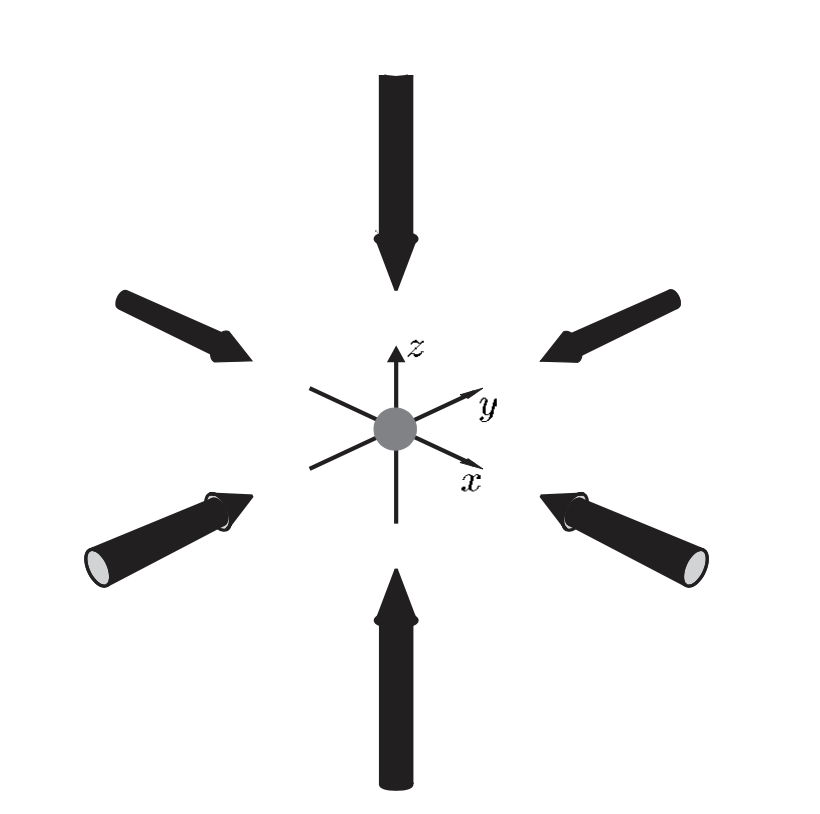
\epsfig{file=fig_optical_molasses.png, scale = .5}
\end{center}
\caption{An set up to create optical molasses.\cite{foot} }
\end{figure}

It is intuitive, since the forces here are velocity dependent, that the result will be a dampening force. This is true and derived in \cite{foot} and \cite{metcalf_article}.
\beq
F_{molasses} = -\beta \nu
\eeq
where the dampening coefficient is of the form
\beq
\beta = 4 \hbar k^2 \frac{I}{I_{sat}} \frac{-2\delta / \Gamma }{\left( 1 + (2\delta / \Gamma )^2 \right)^2}
\eeq

This is a problem if we plan on running this for a long time. This is because the atoms feel no central restoring force. Atoms will leave the optical molasses, hit the side of the structure that encloses them in a vacuum and heat up. For this reason, optical molasses is used for a short period of time once the gas has been cooled to the order of about $100\mu K$. This step in cooling takes advantage of the hyperfine structure of Rubidium-87. \cite{foot}\cite{metcalf_article}\cite{LCandT}

To apply a central restoring force, a magneto-optical trap is used. To build a magneto-optical trap, a magnetic field gradient is applied. This magnetic field splits the energy levels of Rubidium-87 due to the Zeeman effect. This magnetic field, in the NASABEC machine, is formed using quadrupole coils; such that, the strength of the Zeeman splitting, close to the center of the trap, grows as the atoms leave the center of the trap. This splitting for Rubidium-87 can be shown below in \textbf{Figure 1.3}.

\begin{figure}[h!]
\begin{center}
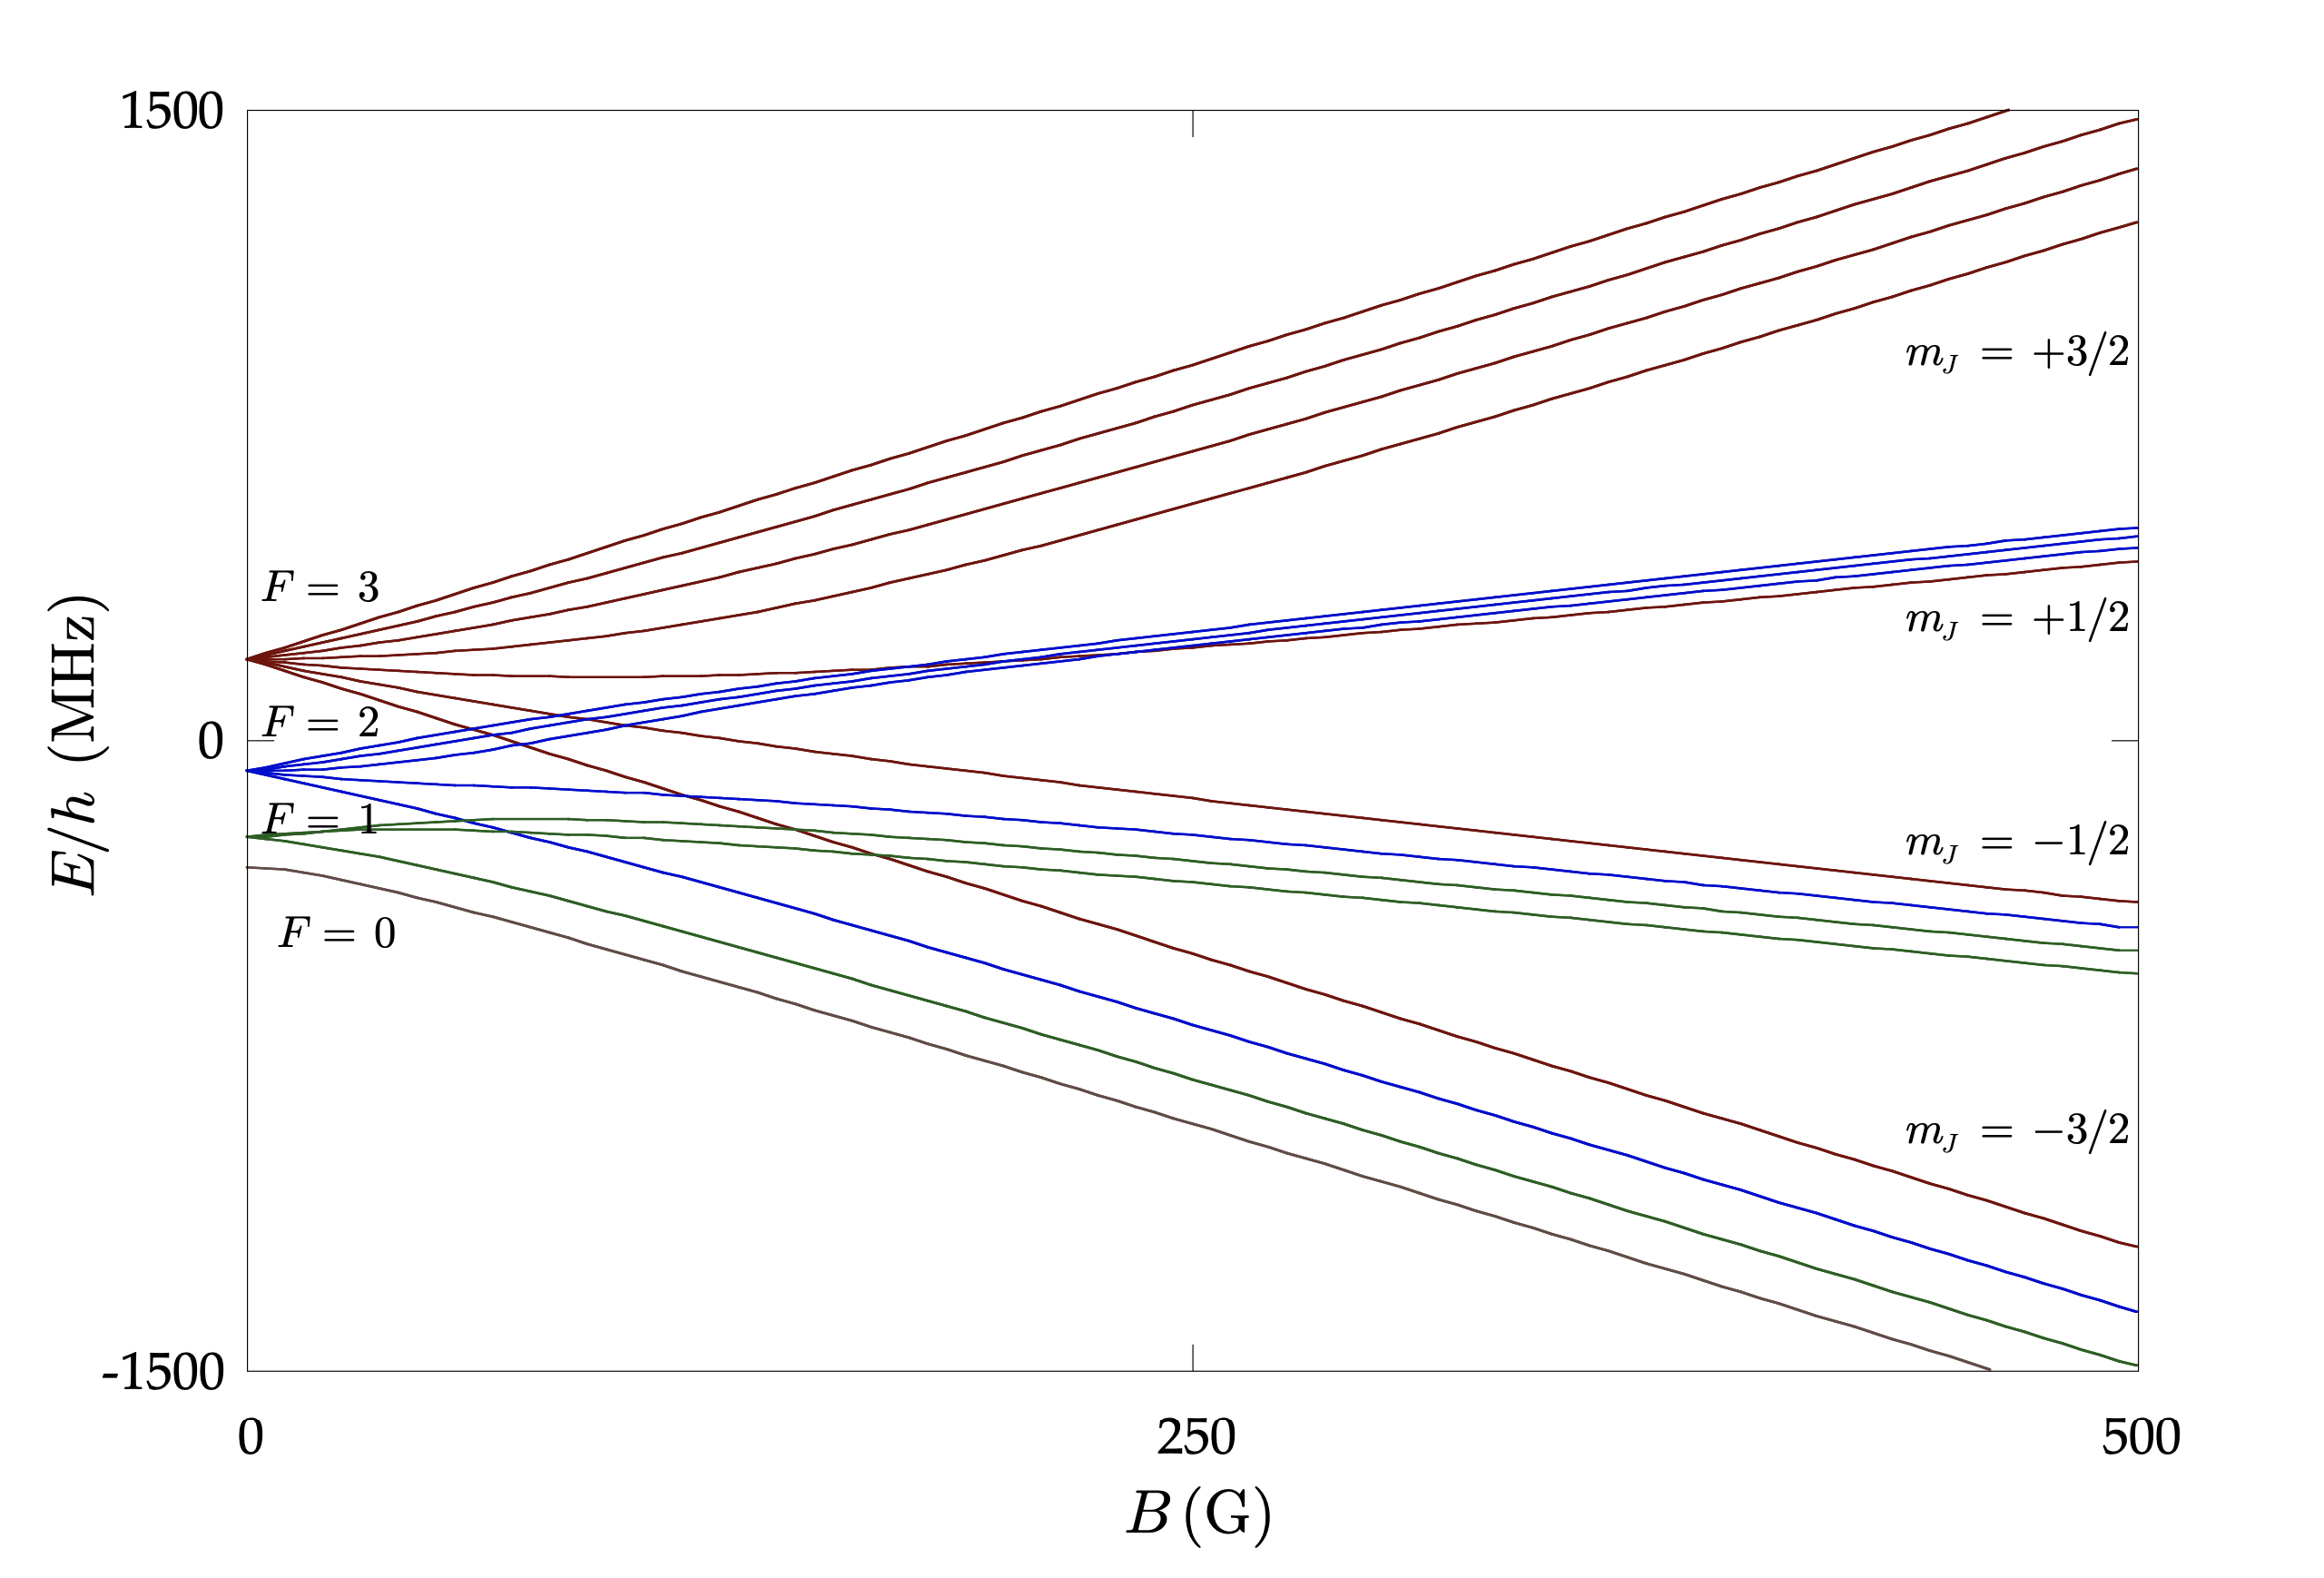
\epsfig{file=fig_zeeman.png, scale = .15}
\end{center}
\caption{The hyperfine structure of Rubidium-87 in an external magnetic field. \cite{steck} }
\end{figure}

Once the hyperfine levels are split, the atoms are exposed to two counter-propagating lasers with different polarizations of light that are red detuned, as shown in \textbf{1.4}. 

\begin{figure}[h!]
\begin{center}
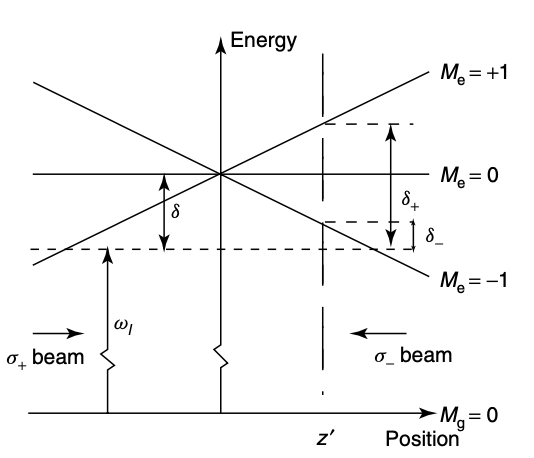
\epsfig{file=fig_MOT.png, scale = .8}
\end{center}
\caption{Visualization of the Zeeman splitting in a magneto-optical trap.   \cite{steck} }
\end{figure}

In a magneto-optical trap, one can imagine two different phenomena occurring. Atoms that are moving fast towards a laser, like in the case of optical molasses, see a light that is more on resonance, so they are more likely to be scattered. In addition, atoms that move away from the center of the trap experience Zeeman splitting. An atom in a position where $z'$ is greater feels a magnetic field that causes the transition where $\Delta M_F = -1$ to become more on resonance and therefore the atoms are more likely to experience a scattering force towards the negative $z'$ direction. When $z'$ is less, the transition where $\Delta M_F = -1$ is more on resonance and so the atom is more likely be scattered to the right by the positive circularly polarized light beam. Formalizing this idea,\cite{foot}

\begin{equation}
        \begin{aligned}[b]
    F_{MOT} &= F_{scatt}^{\sigma^+}(\omega - k\nu - (\omega_0 + \beta z)) - F_{scatt}^{\sigma^-}(\omega + k\nu - (\omega_0 -\beta z)) \\
    & \approx -2 \frac{\partial F}{\partial \omega} k \nu -2 \frac{\partial F}{\partial \omega} \beta z \\
    &= F_{damping} + F_{restoring}
        \end{aligned}
\label{eqn2.qo}
\end{equation}

Under these forces, the atoms undergo over-damped simple harmonic motion. A magneto-optical trap is typically the first step in cooling atoms and is the first step in the NASABEC machine. This machine uses both a two dimensional and three dimensional magneto-optical trap to cool the atoms via a laser. The 2D trap catches heated Rubidium atoms from the air, cooling them. From there atoms leak and are pushed up to the 3D magneto-optical trap which is tuned to be more effective at slowing already cooled atoms to about the Doppler limit, $100 \mu K $. From there, a phase of optical molasses allows for sub-Doppler cooling. The transition for this process in the NASABEC machine is $| F=2\rangle \rightarrow |F'=3\rangle$. Occasionally, while unlikely, atoms will be excited from the $| F=2\rangle$ state to the $| F'=2\rangle$ state and fall down to the $| F=1\rangle$ state. Atoms in the $| F=1\rangle$ state can not be properly cooled. For this reason, a repump beam on resonance with the $| F=1\rangle \rightarrow |F'=2\rangle$ transition is used to repopulate the atoms to the $|F=2\rangle$ state. Over time, the atoms will settle in the $|F=2\rangle$ state, where they can be effectively trapped and cooled. 
\newline

\subsection{Optical Pumping}

The next step in the cooling process is to get a method to trap the atoms without relying on a magneto-optical trap, which will only allow cooling towards the Doppler limit. For this process to be effective the sub-states of the atoms must be purified.

To understand the rules of optical pumping, one must understand the allowed energy level transitions, for which quantum mechanics explain\cite{introQM}. Due to conservation laws, the only transitions that are allowed are those for which $\Delta F = 0, \pm 1$ and $\Delta M_F = 0, \pm 1$. The energy levels for Rubidium-87 can be found as \textbf{Figure A.1} in \textbf{Appendix A}. The hyperfine splitting, the energy difference in the $M_F$ states, is determined by the Zeeman effect.

Hyperfine splitting effects on the required laser frequency are negligible. Controlling transitions for $\Delta F$ is easy as the energy levels vary significantly. The Ultra-Cold Atom Lab uses the $| F=2, M_F = 2\rangle$ state as the trappable state. To understand how the $M_F$ state is purified, a formalization of the polarization of light is helpful.
\newline

\subsubsection{Polarization of Light}
This section will review the concept of light polarization and introduce Jones Vectors. Recall that the polarization of light is described by the direction its electric field points over time. It is known, from the solutions to Maxwell's equations, that the electric field for light is described by 
\beq
\boldsymbol{E}(z,t) = (E_x\boldsymbol{\hat{x}} + E_y \boldsymbol{\hat{y}})e^{i(kz-wt)}
\eeq
\beq
\boldsymbol{E}(z,t) = (|E_x|e^{i\phi_x}\boldsymbol{\hat{x}} + |E_y| e^{i\phi_y}\boldsymbol{\hat{y}})e^{i(kz-wt)}
\eeq
where $k$ is the wave number. Factoring out the effective electric field,
\beq
\boldsymbol{E}(z,t) = E_{eff}(A\boldsymbol{\hat{x}} + B e^{i\delta}\boldsymbol{\hat{y}})e^{i(kz-wt)}
\eeq
where 
\beq
E_{eff} = \sqrt{|E_x|^2 + |E_y|^2}e^{i\phi_x}
\eeq
\beq
A = \frac{|E_x|}{\sqrt{|E_x|^2 + |E_y|^2}}
\eeq
\beq
B = \frac{|E_y|}{\sqrt{|E_x|^2 + |E_y|^2}}
\eeq
\beq
\delta = \phi_y - \phi_x
\eeq
This formalism is helpful as it can describe the proportion of the electric field in the $x$ and $y$ directions using $A$ and $B$. The angle $\delta$ describes the angle between the maximum $E_x$ and $E_y$ components. 

Jones Vectors use the following notation to describe how the electric field propagates:
\beq
\begin{bmatrix} 
A\\
Be^{i\delta}\\
\end{bmatrix} 
\eeq
Using this, the polarization of any plane wave field, which the laser light can be approximated to, can be described. For linearly polarized light, polarized at an angle $\alpha$ from the $x$ axis, the Jones Vector is 
\beq
\begin{bmatrix} 
cos\alpha\\
sin\alpha\\
\end{bmatrix} 
\eeq
For right, or positive, circularly polarized light the Jones Vector is
\beq
\frac{1}{\sqrt{2}}
\begin{bmatrix} 
1\\
-i\\
\end{bmatrix} 
\eeq
In this case, the angle between the maximum $E_x$ component and $E_y$ component differ by a factor of $\frac{\pi}{2}$ and the electric field rotates positively around the axis of propagation. 

A polarizer, a tool that changes the polarization of the light, can be represented as a $2x2$ matrix. A half-wave plate controls the orientation of linearly polarized light. Half-wave plates can be used in conjunction with a beam splitter, an object that lets linear polarized light aligned with its axis pass and reflects the component of light that is not. This is sometimes required because in reality half-wave plates are not perfectly effective. This combination can also split the beam in two paths, where the ratio of light transmitted and reflected can be controlled by changing the axis of linear polarization by turning a half-wave plate. A quarter-wave plate changes linearly polarized light into circularly polarized light and vice versa. The Jones Matrix for a half-wave plate is
\beq
\begin{bmatrix} 
cos2\theta & sin2\theta\\
sin2\theta & -cos2\theta\\
\end{bmatrix} 
\eeq
The Jones Matrix for a quarter-wave plate is
\beq
\begin{bmatrix} 
cos^2\theta +isin^2\theta & (1-i)sin\theta cos\theta \\
(1-i)sin\theta cos\theta & sin^2\theta + icos^2\theta\\
\end{bmatrix} 
\eeq
A quarter-wave plate works by slowing the electric field in one axis until the angle between the maximum $E_x$ and $E_y$ components differ by a factor of $\frac{\pi}{2}$. The magnitude of this phase difference depends on the thickness of the wave plate, $d$, and its refractive index along each axis, which is achieved in the way the crystal is cut. 
\beq
k_{slow}d - k_{fast} d = \frac{\pi}{2} +2\pi m
\eeq
For a half-wave plate
\beq
k_{slow}d - k_{fast} d = \pi +2\pi m
\eeq
where $m$ is any integer. When $m=0$, the wave plate is referred to as a zero order waveplate. A zero order wave plate tends to be more effective in practice. The Ultra-Cold Atom uses all of these optical tools to control the polarization and transmission of laser light as will be shown in \textbf{Chapter 3}.
\newline


\subsubsection{Optical Pumping of Rubidium-87}
\textbf{Figure 1.5} shows the allowed state transitions, where the transition the laser is on resonance with is the $| F=2\rangle \rightarrow |F'=3\rangle$ transition. 


\begin{figure}[h!]
\begin{center}
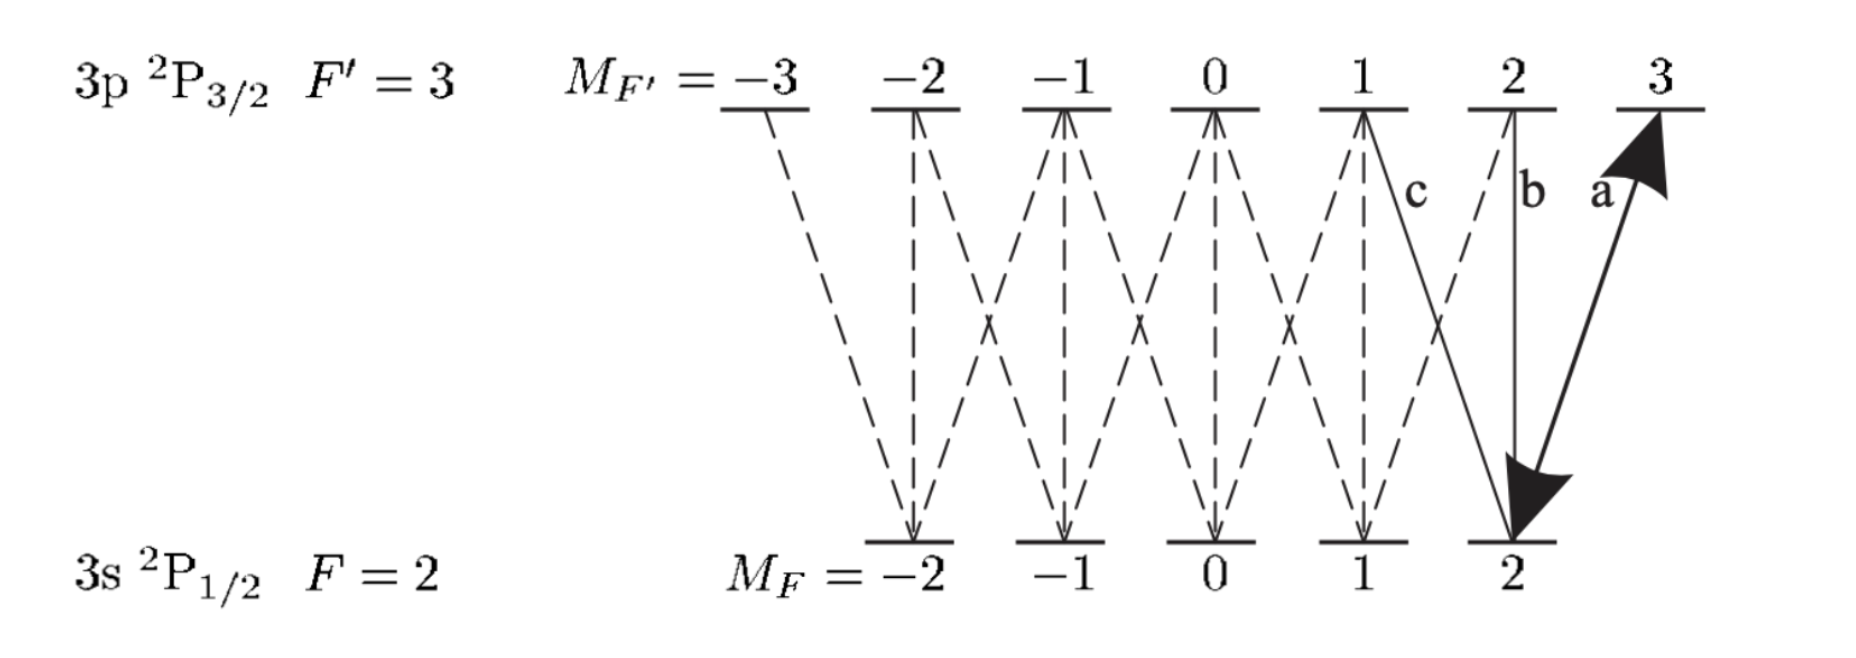
\epsfig{file=fig_allowed_transitions.png, scale = .5}
\end{center}
\caption{The allowed transitions between $| F=2\rangle \rightarrow |F'=3\rangle$. \cite{foot} }
\end{figure}

In addition, only positive circularly polarized light, $\sigma^+$, is used to pump the atoms. The axis of propagation is aligned with the applied external magnetic field so that the dipole moments of the atoms are aligned such that the atoms see positive circularly polarized light without a superposition of linearly polarized light or negative circularly polarized light. Doing this ensures that $\Delta M_F = 1$. Doing this, the atoms eventually begin to settle into the $M_F=2$ substate. With one scatter, the atoms either keep the same state, if $\Delta M_F = -1$ when they fall down to $F=2$, or increase their substate. Once in the $| F=2, M_F = 2\rangle$ state, atoms cycle between the $| F=2, M_F = 2\rangle$ and the $| F'=3, M'_F = 3\rangle$ states. Excessive scattering causes unnecessary heating of the atoms. This process is very fast so the laser must be detuned to not heat the sample. This is explored in \textbf{Chapter 2}. \textbf{Figure 1.6} shows the relative probabilities when driving transitions from the $| F=2\rangle$ state with $\sigma^+$ light.

\begin{figure}[h!]
\begin{center}
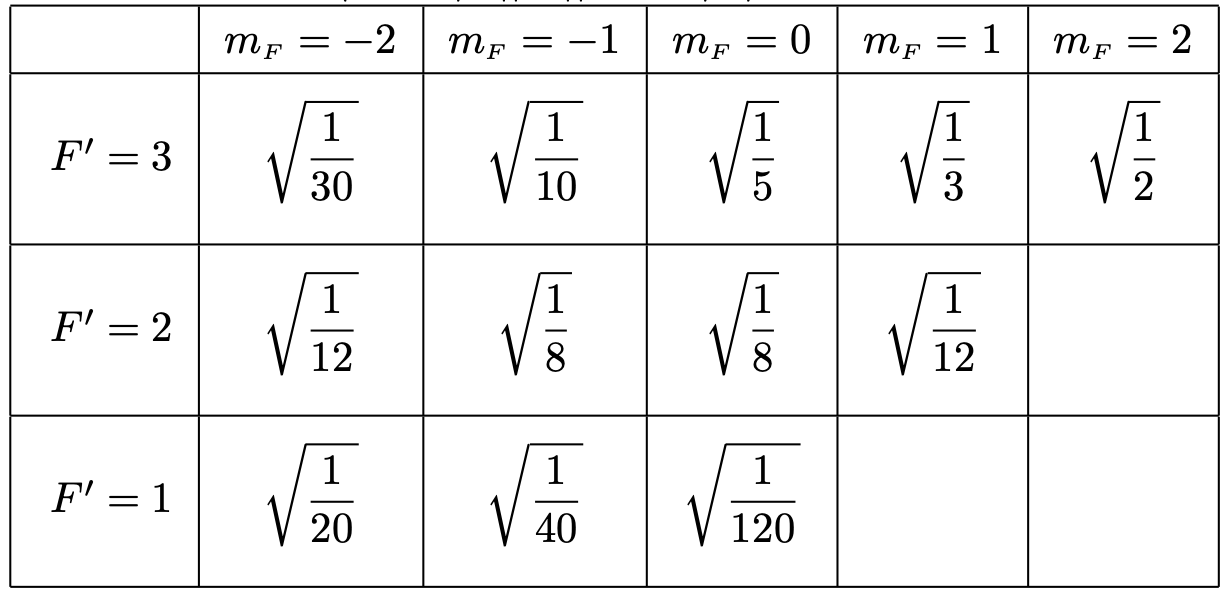
\epsfig{file=fig_trans_table.png, scale = .5}
\end{center}
\caption{The relative probabilities for transitions from $F=2$ with $\sigma^+$ light. \cite{steck} }
\end{figure}

Squaring and doubling these probabilities gives the absolute probabilities between transitions. 
\begin{figure}[h!]
\begin{center}
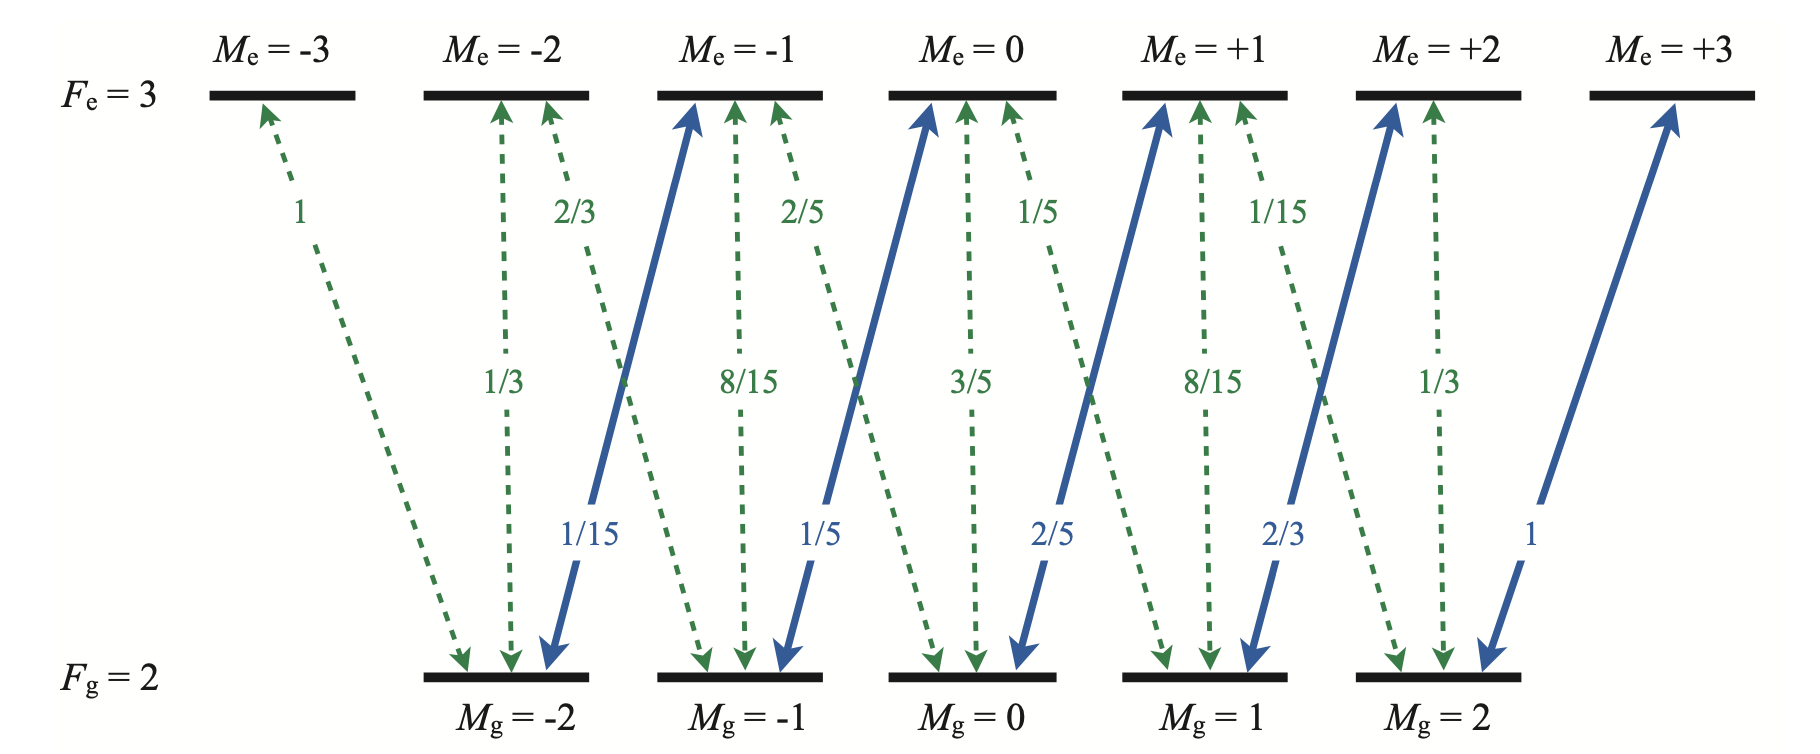
\epsfig{file=fig_rel_probabilities.png, scale = .5}
\end{center}
\caption{The relative probabilities for transitions between $F=2$ and $F'=3$ with $\sigma^+$ light. \cite{Atoneche} }
\end{figure}

Once most of the atoms are purified into the $| F=2, M_F = 2\rangle$ state, they can be effectively trapped by a magnetic trap tailored to capture atoms with the corresponding magnetic dipole. Originally, had the magnetic trap been turned on without optical pumping, states where $M_F$ is negative would be repulsed. Atoms with $M_F=0$ would not feel any force and succumb to gravity. Atoms where $M_F=1$ would not experience as strong of a trapping force and therefore could leak out of the trap with their sufficiently large kinetic energies. Optical pumping purifies the atoms to ensure that they are effectively trapped. 
%%could talk about leakage, probably uneccessary tho

\subsection{Evaporative Cooling}
The final step in Bose-Einstein Condensation formation is evaporative cooling. Evaporative cooling works by removing the atoms with the highest thermal energy to decrease the temperature of the atom cloud by multiple orders of magnitude. This process requires a mechanism to biasedly remove the hottest atoms and a sufficiently high energy transfer rate to reestablish thermal equilibrium. This must be done without decreasing the density of the atoms so that the phase space density increases until the atoms form a Bose-Einstein Condensate. This process is similar the a way a hot cup of coffee cools off, where the hottest atoms evaporate off. 

At this stage, the temperature distribution of the gas can be well approximated by a Boltzmann distribution.
\beq
N(E) = N_0e^{-E/k_bT_1}
\eeq 
where $N(E)$ is the number of atoms with an energy $E$ and $T_1$ is the characteristic temperature. From this distribution, a cutoff energy is chosen and atoms with energies higher than that energy are removed from the trap in a mechanism discussed later. This is referred to as using an RF-knife (radio-frequency). From there, thermal equilibrium is reestablished and a lower cutoff energy is chosen. This process is repeated until the cloud reaches a temperature on the order of about $100nK$ and a Bose-Einstein Condensate is formed. In practice, the process is more continuous as thermal equilibrium is reached sufficiently fast. 

\begin{figure}[h!]
\begin{center}
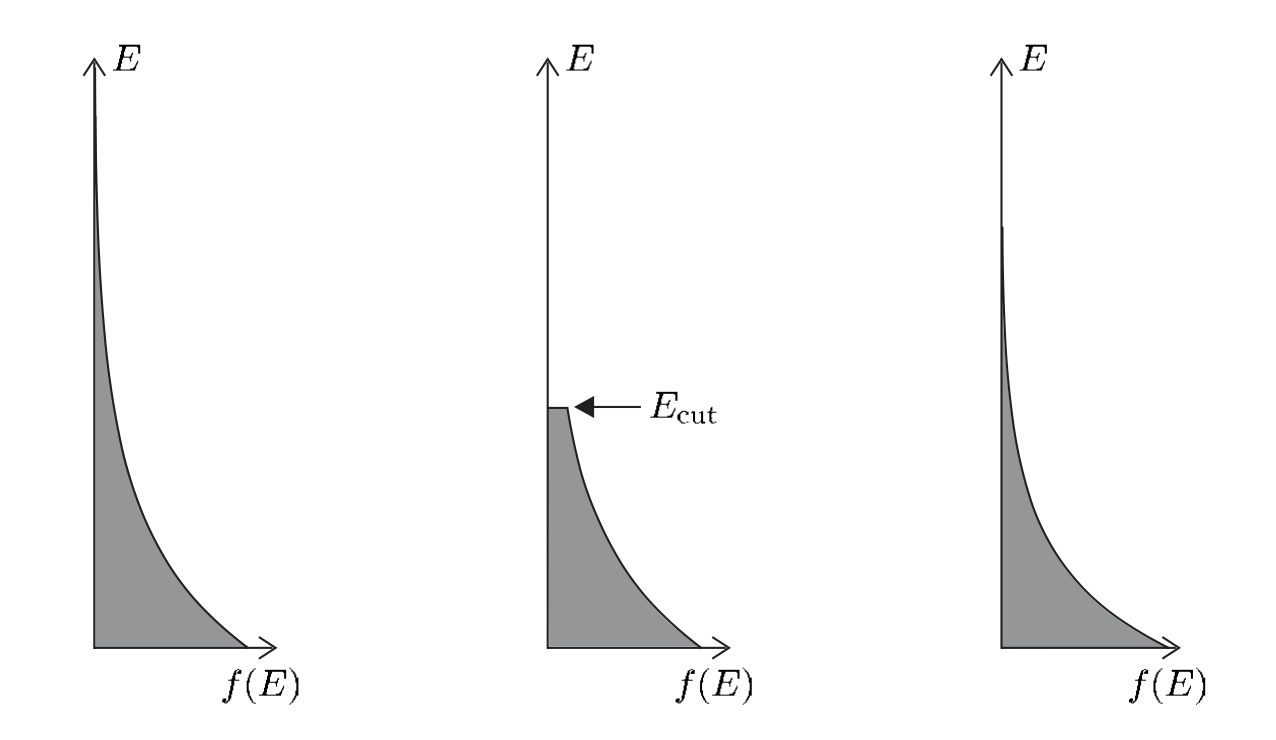
\epsfig{file=fig_e_cutoff.png, scale = .5}
\end{center}
\caption{A visualization of the evaporative cooling process. $f(E)$ is the energy density defined by a Boltzmann distribution. \cite{foot} }
\end{figure}

This mechanism uses what is known as an RF-knife. For this to work, and to keep the phase density of the atoms high, the strength of the magnetic trap is greatly increased. From there, the quadratic Zeeman effect is no longer negligible. The substates of the $|F=2\rangle$ state spread more dramatically as the atoms leave the from the center of the trap. Atoms with higher kinetic energies reach the further edges of the trap as only they have enough energy to overcome the stronger magnetic potential energy. When an atom is farther from the center of the trap its $M_F$ states become more separated as shown in \textbf{Figure 1.9}. 
\begin{figure}[h!]
\begin{center}
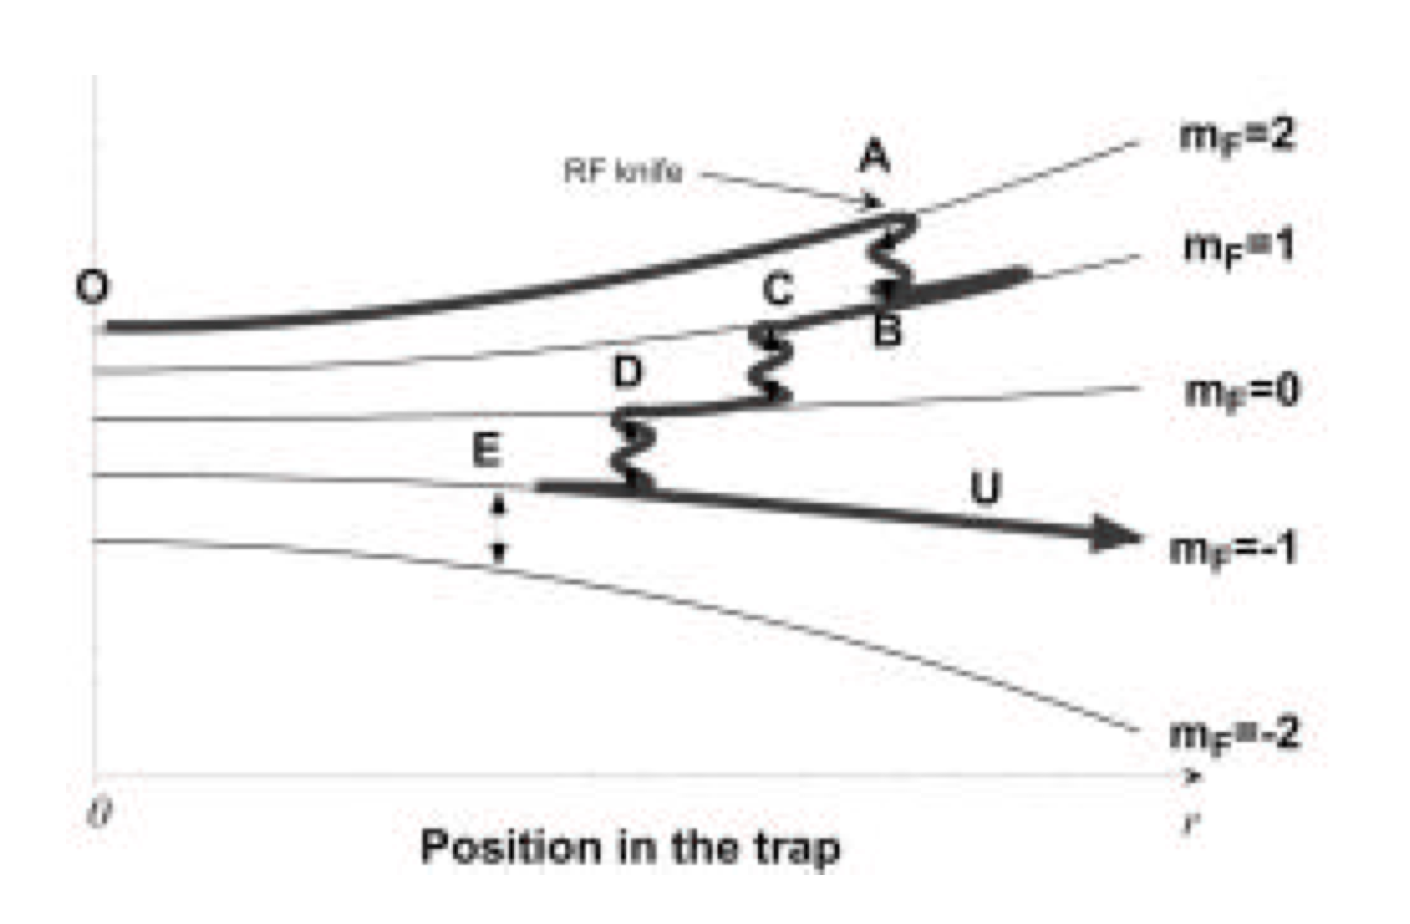
\epsfig{file=fig_quad_zeeman.png, scale = .3}
\end{center}
\caption{A visualization an atom above $E_{cut}$ being removed from the trap. \cite{bouyer} }
\end{figure}

The atoms are exposed to radio frequency light that is tuned such that it is only on resonance for an atoms whose $M_F$ states are sufficiently separated like the difference between \textbf{A} and \textbf{B} in \textbf{Figure 1.9}. At that point, the atom can be excited into lower sub-levels, as the atoms move around the trap, until the magnetic trap forces it out of the trap when $M_F=-1$. The result is not always as shown. An atoms could be re-excited back into a higher energy state should it be the correct distance from the center of the trap. Nonetheless, atoms with sufficiently high energies will eventually be removed from the trap. This final step is repeated until a Bose-Einstein Condensate is formed. 